% !TeX root = RJwrapper.tex
\title{Multivariate Subgaussian Stable Distributions in R}
\author{by Bruce J. Swihart, John P. Nolan}

\maketitle

\abstract{ We introduce and showcase \CRANpkg{mvpd} (an acronym for
  \emph{m}ulti\emph{v}ariate \emph{p}roduct \emph{d}istributions), a
  package that uses a product distribution approach to calculating
  multivariate subgaussian stable distribution functions.  The family
  of multivariate subgaussian stable distributions are elliptically
  contoured multivariate stable distributions that contain the
  multivariate Cauchy and the multivariate normal distribution. These
  distributions can be useful in modeling data and phenomena that have
  heavier tails than the normal distribution (more frequent occurrence
  of extreme values).  Application areas include log returns for
  stocks, signal processing for radar and sonar data, astronomy, and
  hunting patterns of sharks. }

\section{Introduction}

% \begin{figure}[htbp]
%   \centering
%   \includegraphics[scale=0.45]{CRAN_task_view}
%   \caption{CRAN Task View: Probability Distributions screenshot
%   \label{fig:taskview}}
% \end{figure}


Multivariate subgaussian stable distributions are the elliptically
contoured subclass of general multivariate stable distributions.  To
begin a brief introduction to multivariate subgaussian stable
distributions, we start with univariate stable distributions which may
be more readily familiar and accessible. Univariate stable
distributions are a flexible family and have four parameters,
$\alpha$, $\beta$, $\gamma$, and $\delta$, and at least eleven
parameterizations (!)  which has led to much confusion
\citep{nolan2020univariate}.  Here we focus on the 1-parameterization
of the Nolan style. Location is controlled by $\delta$, scale by
$\gamma \in (0,\infty)$, while $\alpha \in (0,2]$ and
$\beta \in [-1,1]$ can be considered shape parameters.  Being a
location-scale family, a ``standard" stable distribution will be when
$\gamma=1$ and $\delta=0$. A solid introduction to univariate stable
distributions can be found in the recent textbook \emph{Univariate
  Stable Distributions} \citep{nolan2020univariate} and its freely
available Chapter 1 online
(\url{https://edspace.american.edu/jpnolan/stable/}).

\begin{figure}
  \center
  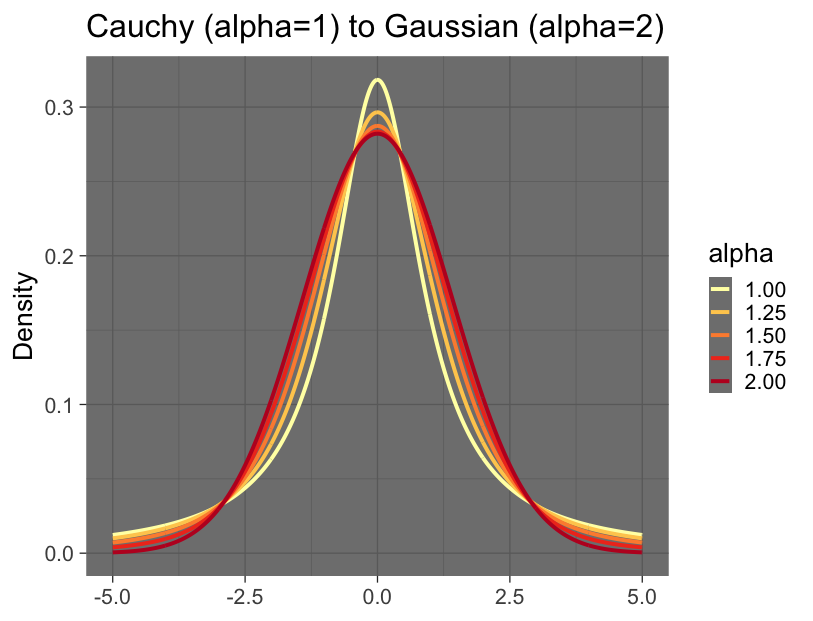
\includegraphics[scale=.4]{cauchy2gauss.png}
%  \caption{Standard univariate subgaussian distributions for various
%    values of alpha.  Cauchy is alpha=1 and normal is alpha=2.}
  \caption{The lower the value of alpha, the heavier the tails.
The superimposed standard univariate subgaussian densities for
selected values of alpha are displayed.  Commonly known distributions
include the Cauchy (alpha=1) and normal (alpha=2).}
  \label{fig:univariate}
\end{figure}

Univariate symmetric stable distributions are achieved by setting the
skew parameter $\beta=0$, which gives symmetric distributions that are
bell-shaped like the normal distribution.  A way to remember that
these are called subgaussian is to see that as $\alpha \in (0,2]$
increases from 0 it looks more and more normal until it \strong{is}
normal for $\alpha=2$ (Figure~\ref{fig:univariate}).  The \emph{sub}
in subgaussian refers to the tail behavior in that the rate of
decrease in the tails is \emph{less} than that of a gaussian -- note
how the tails are above the gaussian for $\alpha<2$ in
Figure~\ref{fig:univariate}.  Equivalently, as $\alpha$ decreases, the
tails get heavier.  A notable value of $\alpha$ for subgaussian
distributions is $\alpha=1$ which is the Cauchy distribution.  The
Cauchy and Gaussian distribution are most well-known perhaps because
they have closed-form densities, which all other univariate symmetric
stable distributions lack.

% The
% Gaussian is more well-known than the Cauchy perhaps because it has a
% finite variance whereas the Cauchy does not.  In fact, the Cauchy
% doesn't have a defined 1st moment either.  
Therefore, numerically computing the densities is especially important
for application.  For univariate stable distributions, there is
open-source software to compute modes, densities, distributions, quantiles
and random variates, including a number of R packages
(\CRANpkg{stabledist}, \CRANpkg{stable}, \CRANpkg{libstableR}, for
example -- see CRAN Task View: Probability \ctv{Distributions} for
more).


As generalizations of the univariate stable distribution, multivariate
stable distributions are a very broad family encompassing many
complicated distributions (e.g. support in a cone, star shaped level
curves, etc.).  A subclass of this family is the
multivariate subgaussian stable distributions. Multivariate
subgaussian stable distributions are symmetric and elliptically
contoured.  Similar to the aforementioned univariate symmetric stable
distributions, the value $\alpha=2$ is the multivariate gaussian and
$\alpha=1$ is the multivariate Cauchy.  Being that they are
elliptically contoured and symmetric makes them applicable to finance
where joint returns have an (approximately) elliptical joint
distribution \citep{nolan2020univariate}.  Signal processing, such as
with radar and sonar data, tasks itself with filtering impulsive noise
from a signal of interest and linear filters in the presence of
extreme values tend to underperform, whereas using multivariate stable
distributions have been fruitful \citep{tsakalides1998deviation,
  nolan2013multivariate}.  The (multivariate) Holtsmark distribution
is a multivariate subgaussian stable distribution ($\alpha=1.5$) that
has applications in astronomy, astrophysics, and plasma
physics. L{\'e}vy flights, which are random walks with steps having a
specific type of multivariate subgaussian stable distribution, are
used to model interstellar turbulence as well as hunting patterns of
sharks \citep{boldyrev2003levy, sims2008scaling}.


For multivariate subgaussian stable distributions, the parameter
$\alpha$ is a scalar as in the univariate family, while
$\boldsymbol{\delta}$ (location) becomes a $d$-dimensional vector and
the analogue for the scale parameter is a $d \times d$ shape matrix
$Q$. The shape matrix $Q$ needs to be semi-positive definite and is
neither a covariance matrix nor covariation matrix.  An introduction
to multivariate subgaussian stable distributions can be found in
\citet{nolan2013multivariate}.


Including \CRANpkg{mvpd}, the focus of this paper, if one wanted
\code{R} functions to interact with multivariate subgaussian stable
distributions they have three \code{R} package options. These packages
are compared in Table~\ref{tab:checkmark} and detailed below:

\begin{itemize}

\item \CRANpkg{alphastable} provides random univariate and multivariate generation, density
  calculation, and parameter fitting (albeit for modest sample sizes)
  via an EM algorithm method \citep{teimouri2018,
  alphastableRpackage}.

\item \pkg{stable} provides support for all stable univariate
  distributions and multivariate subgaussian stable distributions.
  Other cases are handled, to varying degrees, such as isotropic,
  independent, and spectral measure.  For the purposes of this paper,
  we will note that the \pkg{stable} package provides random variate
  generation, density calculation, parameter fitting, distribution
  calculations via Monte Carlo methods for multivariate subgaussian
  stable distributions $2 \leq d \leq 100$. The \pkg{stable} package
  is developed by Robust Analysis and is available for purchase or
  through a software grant at \url{http://www.robustanalysis.com/}.
  It is distinct from the univariate \CRANpkg{stable} package on CRAN
  authored by Jim Lindsey.

\item \CRANpkg{mvpd} provides random variate generation, density
  calculation, parameter fitting, distribution function calculations via
  Monte Carlo methods, as well as an integrated method for distribution
  calculations that allows tolerance specification.

\end{itemize}



%% x's for lack of functionality
\begin{table}[]
  \begin{tabular}{l|ccc}
 Functionality  & \code{alphastable} & \code{stable}  & \code{mvpd}\\
\hline
random variates & \checkmark  & \checkmark  & \checkmark  \\
parameter estimation  & \checkmark  & \checkmark  & \checkmark  \\
density  & \checkmark  & \checkmark  & \checkmark  \\
cumulative distribution (monte carlo) & x & \checkmark & \checkmark \\
cumulative distribution (integrated) & x & x & \checkmark \\
multivariate subgaussian stable& \checkmark  & \checkmark & \checkmark \\
 multivariate independent stable & x  & \checkmark  & x \\
  multivariate isotropic stable & x & \checkmark  & x \\
   multivariate discrete-spectral-measure stable & x & \checkmark  & x
  \end{tabular}
  \caption{\label{tab:checkmark} Summary of functionality among
    \code{R} packages.  Note: The \code{stable} package referenced is
    not the one on CRAN -- it is proprietary software produced by the
    company Robust Analysis.}
\end{table}


  
While the lack of a tractable density and distribution function
impedes directly calculating multivariate subgaussian stable
distributions, it is possible to represent them in terms of a product
distribution for which each of the two distributions in the product
has known numerical methods developed and deployed (in \code{R}
packages on CRAN). This paper utilizes this approach.  The next
section covers some product distribution theory.


% Section~\ref{sect:pdt} covers some
% light product distribution theory.
%% and gives two pertinent examples.
% Implementation in R is covered in Section~\ref{sect:imp} and
% accuracy and computation time are considered for some scenarios in
% Section~\ref{sect:acctime:setup} with the results in
% Section~\ref{sect:acctime:results}.


\section{Product distribution theory \label{sect:pdt}}

This section reviews some known results of \emph{product
distributions} and describes our notation.  Allow univariate positive
random variable $A$ with density $f_A(x)$ and $d$-dimensional random
variable G to have density $f_G(\bm{x})$ and distribution function
$F_G(\bm{v}, \bm{w}) = P( \bm{v} < \bm{x} \leq \bm{w})$.  Consider the
$d-$dimensional product $H=A^{1/2} G$.  From standard product
distribution theory we know the density $f_H$ is represented by
1-dimensional integral:

\begin{eqnarray}
f_{H}(\bm{x}) &=& \int_0^{\infty} f_B(u) f_G(\bm{x} / u)
\frac{1}{|u|^d} du \,, \label{eq:density:general}
\end{eqnarray}
where $B=A^{1/2}$ so that $f_B(x) \coloneqq 2 x f_A(x^2)$.
Consequently the distribution function $F_H$ (with lower bound $\bm{v}$ and
upper bound $\bm{w}$) of the r.v. $H$ is represented by

\begin{eqnarray}
F_{H}(\bm{v}, \bm{w}) 
&=& \int_0^{\infty} 
f_B(u) 
\int_{v_1}^{w_1} \dots \int_{v_d}^{w_d}  f_G(\bm{t} / u) \frac{1}{|u|^d} dt_1 \dots dt_d
du \,, \\
&=& \int_0^{\infty} 
f_B(u) 
\int_{v_1 / u}^{w_1 / u} \dots \int_{v_d / u}^{w_d / u}  f_G(\bm{t})
dt_1 \dots dt_d du \,, \nonumber \\
&=& \int_0^{\infty} 
f_B(u) F_G(\bm{v} / u, \bm{w}/u) du. \label{eq:distribution:general}
\end{eqnarray}
Take note of the representation in (\ref{eq:density:general}) and (\ref{eq:distribution:general}).  From
a practical standpoint, if we have a (numerical) way of calculating
$f_A$, $f_G$, and $F_G$ we can calculate $f_H$ and $F_H$.  Different
choices can be made for $f_A$, $f_G$, and $F_G$ in this general
setup.  The choices required for multivariate subgaussian stable
distributions are covered in the following Implementation section.

\subsection{Multivariate elliptically contoured stable distributions \label{sect:A:stable}}

From \citet{nolan2013multivariate}, $H$ is a $d$-dimensional
subgaussian stable distribution if $A$ is a positive univariate stable distribution
$$A \sim S\left( \frac{\alpha}{2}, 1, 2 \cos \left( \frac{\pi
      \alpha}{4} \right)^{\left(\frac{2}{\alpha}\right)} , 0;
  1\right)$$ and $G$ is a $d$-dimensional multivariate normal
$G \sim MVN( 0, Q)$, where the shape matrix $Q$ is positive semi-definite.
This corresponds to Example 17 in \citet{hamdan2000characterizing}.


\section{Implementation \label{sect:imp}}
Using the aforementioned theory of product distributions, we can
arrive at functions for a multivariate subgaussian stable density and
distribution function thanks to established functions for univariate
stable and multivariate normal distributions. A key package in the
implementation of multivariate subgaussians in R is \CRANpkg{mvtnorm}
\citep{mvtnorm2020package, mvtnorm2009book}. In the basic
product-distribution approach of \CRANpkg{mvpd}, $f_G$ and
$F_G$ are \code{mvtnorm::dmvnorm} and \code{mvtnorm::pmvnorm}
respectively.  Allow the density of $A$, $f_A$ (to be numerically
calculated in \code{R}) using \code{stable::dstable} or
\code{libstableR::stable\_pdf}  \citep{libstableRpackage}. Presented as pseudo-code:

\begin{itemize}

% \item $f_A(x, \alpha) \coloneqq \texttt{stabledist::dstable}(x,
%   \frac{\alpha}{2}, 1, 2 \cos \{ \frac{\pi \alpha}{4}
%   \}^{\left(\frac{2}{\alpha}\right)}   , 0; \texttt{pm=1})$

\item $f_A(x, \alpha) \coloneqq \texttt{libstableR::stable\_pdf}(x,
  \texttt{pars = } \left(\frac{\alpha}{2}, 1, 2 \cos \{ \frac{\pi \alpha}{4}
  \}^{\left(\frac{2}{\alpha}\right)}   , 0\right); \texttt{pm = 1})$


% \item $f_A(x, \alpha) \coloneqq$
%  \code{(x, libstableR::stable\_pdf(x, pars=c(alpha = alpha/2,
%                                         beta = 1,
%                                         sigma = 2*cos(pi*alpha/4)^(2/alpha),
%                                         mu = 0),
%                                         parametrization = 1L)}
  
\item $f_B(x, \alpha) \coloneqq 2 x f_A(x^2, \alpha)$

\item $f_{H}(\bm{x}, \alpha, Q) = \int_0^{\infty} f_B(u; \alpha)
  \times  \texttt{mvtnorm::dmvnorm}(\bm{x} / u, {\rm sigma}= Q) \frac{1}{|u|^d} du$

\item $F_{H}(\bm{v}, \bm{w}, \alpha, Q) = \int_0^{\infty} 
f_B(u; \alpha) \times 
\texttt{mvtnorm::pmvnorm}({\rm lower} =\bm{v}/u, {\rm upper}=\bm{w}/u,
{\rm sigma}=Q) du$ 
\end{itemize}

The (outermost) univariate integral is numerically evaluated with
\code{stats::integrate}.

\pagebreak

\section{Quick start}

We present an outline of the \code{[dpr]mvss}
(\emph{m}ulti\emph{v}ariate \emph{s}ubgaussian \emph{s}table)
functions, and walk through the code in the subsequent sections. As an
overview, we generate 5000 5-dimensional subgaussian variates with
$\alpha=1.7$ and an ``exchangeable'' shape matrix using \code{rmvss}.
We then recover the parameters with an illustrative call to
\code{fit\_mvss}. We can calculate the density (\code{dmvss}) at the
center of the distribution and get a quick estimate of the
distribution between -2 and 2 for each member of the 5-dimensional
variate using \code{pmvss\_mc}.  We investigate a refinement of that
quick distribution estimate using \code{pmvss}.

% \begin{example}
% library(mvpd)
% set.seed(10)
% shape_matrix <- structure(c(1, 0.9, 0.9, 0.9, 0.9,
%                             0.9, 1, 0.9, 0.9, 0.9,
%                             0.9, 0.9, 1, 0.9, 0.9,
%                             0.9, 0.9, 0.9, 1, 0.9,
%                             0.9, 0.9, 0.9, 0.9, 1),
%                           .Dim = c(5L, 5L))
% X <- mvpd::rmvss(n=5000, alpha=1.7, Q=shape_matrix)
% copula::pairs2(X)
% fitmv <- mvpd::fit_mvss(X)
% fitmv
% mvpd::dmvss(x=fitmv$univ_deltas,
%             alpha=fitmv$mult_alpha, 
%             Q=fitmv$mult_Q_posdef,
%             delta=fitmv$univ_deltas)[1]
% mvpd::pmvss_mc(lower=rep(-2,5),
%                upper=rep( 2,5),
%                alpha=fitmv$mult_alpha,
%                Q=fitmv$mult_Q_posdef,
%                delta=fitmv$univ_deltas,
%                n=10000)
% mvpd::pmvss(lower=rep(-2,5),
%             upper=rep( 2,5),
%             alpha=fitmv$mult_alpha,
%             Q=fitmv$mult_Q_posdef,
%             delta=fitmv$univ_deltas,
%             abseps.pmvnorm = 1e-4,
%             maxpts.pmvnorm = 25000*10,
%             abs.tol.si = 1e-2)[1]

% \end{example}


\section{Random variates generation with \code{rmvss}}

We'll generate 5000 $5$-dimensional subgaussian random variates with a
specified $\alpha$ and shape matrix. They are pictured in
Figure~\ref{fig:scatter}. In the next section we will fit a
distribution to these.

\begin{example}
  R> library(mvpd)
  ## reproducible research sets the seed
  R> set.seed(10)
  ## specify a known 5x5 shape matrix
  R> shape_matrix <- structure(c(1, 0.9, 0.9, 0.9, 0.9,
                                 0.9, 1, 0.9, 0.9, 0.9,
                                 0.9, 0.9, 1, 0.9, 0.9,
                                 0.9, 0.9, 0.9, 1, 0.9,
                                 0.9, 0.9, 0.9, 0.9, 1),
                                 .Dim = c(5L, 5L))
  ## generate 5000 5-dimensional random variables
  ## with alpha = 1.7 and shape_matrix                               
  R> X <- mvpd::rmvss(n = 5000, alpha = 1.7, Q = shape_matrix)
  ## plot all pairwise scatterplots (Figure 2)                            
  R> copula::pairs2(X)
\end{example}

\begin{figure}
  \center
  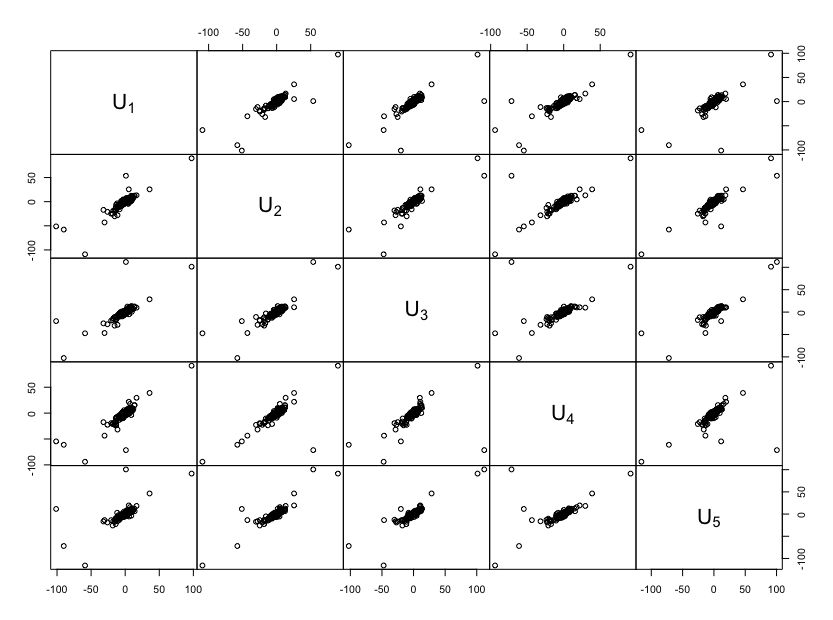
\includegraphics[scale=0.4]{copulascatter.png}
%  \caption{A lattice of scatterplots of the 5-dimensional subgaussian
%    stable distribution.}
  % \caption{A lattice of scatterplots of 5,000 draws from a 5-dimensional subgaussian
  %   stable distribution, showing the pairwise relations.  The outliers
  %   from the cloud in each plot demonstrate the heavy tails.  The tilt
  %   of the cloud along the 45 degree line shows the positive pairwise
  %   association. A multivariate normal with the same shape matrix
  %   would rarely have absolute values bigger than 5, here we see
  %   values upwards of 100.}
\caption{A lattice of scatterplots of 5,000 draws from a 5-dimensional subgaussian
    stable distribution, showing the pairwise relations.  The outliers
    from the cloud in each plot demonstrate the heavy tails.}
  \label{fig:scatter}
\end{figure}


The ability to simulate from a distribution is useful for running
simulations to test different scenarios about the phenomena being
modeled by the distribution, as well as in this case, to generate a
dataset with a known shape matrix and alpha to show our fitting
software (next section) can recover these parameters.  Our quick start
code begins with generating a dataset from a known alpha and shape
matrix. However, often a practitioner might start with a dataset from
which parameters are estimated and then random samples can be
generated from the distribution specified with those parameters to
learn more about the data generating distribution and the behavior of
the phenomena.

\section{Fitting a multivariate subgaussian distribution with
  \code{fit\_mvss}}

If you have data in a $n \times d$ matrix $\bold{X}$ and want to fit a
$d$-dimensional multivariate subgaussian distribution to those data,
then \code{fit\_mvss} will return estimates of the parameters using
the method outlined in \cite{nolan2013multivariate}.  The method
involves fitting univariate stable distributions for each column and
assessing the resulting $\alpha$, $\beta$ and $\delta$ parameters.
The column-wise $\alpha$ estimates should be similar and the
column-wise $\beta$ estimates close to 0.  This column-wise univariate
fitting is carried out by \code{libstableR::stable\_fit\_mle2d(W,
  parametrization = 1L)} and the off diagonal elements can be found
due to the properties of univariate stable distributions (see
\cite{nolan2013multivariate}).  For your convenience, the univariate
column-wise estimates of $\alpha$, $\beta$, $\gamma$ and $\delta$ are
returned in addition to the raw estimate of the shape matrix and the
nearest positive definite shape matrix (as computed by
\code{Matrix::nearPD} applied to the raw estimate).

\begin{example}
  ## take X from previous section and estimate
  ## parameters for the data generating distribution
  R> fitmv <- mvpd::fit_mvss(X)
  R> fitmv
  $univ_alphas
  [1] 1.698617 1.708810 1.701662 1.696447 1.699372
  
  $univ_betas
  [1] -0.02864287 -0.04217262 -0.08444540 -0.06569907 -0.03228573
  
  $univ_gammas
  [1] 1.016724 1.000151 1.008055 1.012017 1.002993
  
  $univ_deltas
  [1] -0.03150732 -0.06525291 -0.06528644 -0.07730645 -0.04539796
  
  $mult_alpha
  [1] 1.700981
  
  $mult_Q_raw
            [,1]      [,2]      [,3]      [,4]      [,5]
  [1,] 1.0337276 0.9034599 0.8909654 0.8937814 0.8647089
  [2,] 0.9034599 1.0003026 0.9394846 0.9072368 0.8535091
  [3,] 0.8909654 0.9394846 1.0161748 0.8929937 0.9037467
  [4,] 0.8937814 0.9072368 0.8929937 1.0241777 0.9281714
  [5,] 0.8647089 0.8535091 0.9037467 0.9281714 1.0059955

  $mult_Q_posdef
            [,1]      [,2]      [,3]      [,4]      [,5]
  [1,] 1.0337276 0.9034599 0.8909654 0.8937814 0.8647089
  [2,] 0.9034599 1.0003026 0.9394846 0.9072368 0.8535091
  [3,] 0.8909654 0.9394846 1.0161748 0.8929937 0.9037467
  [4,] 0.8937814 0.9072368 0.8929937 1.0241777 0.9281714
  [5,] 0.8647089 0.8535091 0.9037467 0.9281714 1.0059955
\end{example}  



An alternative for fitting this distribution is
\code{alphastable::mfitstab.elliptical(X, 1.70, shape\_matrix,
rep(0,5))} and takes 8 minutes (and requires initial values for alpha,
the shape matrix, and delta). This analysis with \code{fit\_mvss(X)}
took under 2 seconds.  For a run of \code{n=1e6, d=20},
\code{fit\_mvss} scales well, taking 60 minutes.


Once the distribution has been fitted, \code{fitmv\$mult\_alpha},
\code{fitmv\$mult\_Q\_posdef}, and \code{fitmv\$univ\_deltas}, can be
used as the \code{alpha}, \code{Q}, and \code{delta} arguments,
respectively, in calls to \code{dmvss} to calculate densities
and \code{pmvss\_mc} or \code{pmvss} to calculate
probabilities.  They could also be passed to \code{rmvss} to
generate random variates for simulations.

\section{Density calculations with \code{dmvss}}

We can calculate the density at the center of the distribution.

\begin{example}
  ## density calculation
  R> mvpd::dmvss(x = fitmv$univ_deltas, 
  +              alpha = fitmv$mult_alpha, 
  +              Q = fitmv$mult_Q_posdef,
  +              delta = fitmv$univ_deltas)[1]
  $value
  [1] 0.1278952
\end{example}


\section{Distribution calculation by Monte Carlo with
  \code{pmvss\_mc}}

The method of calculating the distribution by Monte Carlo relies on the
ability to produce random variates quickly and then calculate what
proportion of them fall within the specified bounds.  To generate multivariate
subgaussian stable variates, a scalar A is drawn from
$$\texttt{libstableR::stable\_rnd}(n,
  \texttt{pars = } \left(\frac{\alpha}{2}, 1, 2 \cos \{ \frac{\pi \alpha}{4}
    \}^{\left(\frac{2}{\alpha}\right)}   , 0\right); \texttt{pm = 1})$$
  and then the square-root of $A$ multiplied by a draw $G$ from
$$\texttt{mvtnorm::rmvnorm}(n, {\rm sigma}=Q).$$
This allows for quick
calculations but to increase precision requires generating larger
number of random variates.  For instance, if we wanted the distribution
between -2 and 2 for each dimension, we could generate 10,000 random variates
and then see how many of them fall between the bounds.  It looks like
6,820 variates were within the bounds: 


\begin{example}
  ## first-run of pmvss_mc
  R> mvpd::pmvss_mc(lower = rep(-2,5),
  +                 upper = rep( 2,5),
  +                 alpha = fitmv$mult_alpha,
  +                 Q = fitmv$mult_Q_posdef,
  +                 delta = fitmv$univ_deltas,
  +                 n = 10000)
  [1] 0.6820
\end{example}

We run it again and the answer changes: 

\begin{example}
  ## second-run of pmvss_mc
  R> mvpd::pmvss_mc(lower = rep(-2,5),
  +                 upper = rep( 2,5),
  +                 alpha = fitmv$mult_alpha,
  +                 Q = fitmv$mult_Q_posdef,
  +                 delta = fitmv$univ_deltas,
  +                 n = 10000)
  [1] 0.6742
\end{example}

With the Monte Carlo method, precision is not specified and no error
is calculated. The next section introduces how to use the integrated
distribution function $F_H$ from product theory and specify precision.


\section{Distribution function calculation via integration with \code{pmvss}}

There are three inexact entities involved in the distribution
calculation $F_H$ as found in \code{pmvss}: the numerically
calculated $F_G$, the numerically calculated $f_A$, and the outer
numerical integration.

The outer integral by \code{integrate} assumes the integrand is
calculated without error, but this is not the case.  See the
supplementary materials section ``Thoughts on error propagation in
\code{pmvss}'' for justification and guidance for specifying the
values of \code{abs.tol.si}, \code{abseps.pmvnorm}, and
\code{maxpts.pmvnorm}.  The first of these three arguments is passed
to the \code{abs.tol} argument of \code{stats::integrate} and controls
the absolute tolerance of the numerically evaluated outer
1-dimensional integral.  The remaining two are passed to \code{maxpts}
and \code{abseps} of \code{mvtnorm::GenzBretz} and control the
accuracy of \code{mvtnorm::pmvnorm}.

Briefly, our experience suggests that to be able to treat
\code{abs.tol.si} as the error of the result, \code{abseps.pmvnorm}
should be 1e-2 times smaller than the specified \code{abs.tol.si}
which may require a multiple of the default 25000 default of
\code{maxpts.pmvnorm} -- which will lead to more computational
intensity and longer computation times as demonstrated below (as
conducted on Macbook Intel Core i7 chip with 2.2 GHz):

\begin{example}
## abs.tol.si    abseps.pmnvorm   maxpts         Time
## 1e-01         1e-03            25000
## 1e-02         1e-04            25000*10        3 sec
## 1e-03         1e-05            25000*100      22 sec
## 1e-04         1e-06            25000*1000      4 min
## 1e-05         1e-07            25000*10000    26 min
## 1e-06         1e-08            25000*85000   258 min
\end{example}

With this in mind, the output from the Quick Start code is:

\begin{example}
  ## precision specified pmvss
  R> mvpd::pmvss(lower = rep(-2,5),
  +              upper = rep( 2,5),
  +              alpha = fitmv$mult_alpha,
  +              Q = fitmv$mult_Q_posdef,
  +              delta = fitmv$univ_deltas,
  +              abseps.pmvnorm = 1e-4,
  +              maxpts.pmvnorm = 25000*10,
  +              abs.tol.si = 1e-2)[1]
  $value
  [1] 0.6768467
\end{example}


Both \code{pmvss} and \code{pmvss\_mc} take infinite limits. Since
\code{pmvss\_mc} calculates how many random variates
$H_i,~ i \in \{1,\dots,n\}$ are within the bounds, \code{pmvss} might
be preferred to \code{pmvss\_mc} when calculating the tails of the
distribution, unless $n$ is made massively large.



%\pagebreak



\section{Speed and accuracy trials \label{sect:acctime:setup}}


We provide a sense of accuracy and computational time trade-offs with a
modest simulation experiment (Figure~\ref{fig:speedacc1}, see
supplementary materials for code).  Estimating these distributions is
inherently difficult -- difficult in the sense that expecting accuracy
farther out than the 5th decimal place for distribution functions is
unreasonable.  Therefore, we will define our ``gold standard" targets
for accuracy evaluation as the numerical density produced by Robust
Analysis' \code{dstable} integrated by \code{cubature::hcubature()}
with tolerance \code{tol=1e-5}.


We will time three functions using \code{bench::mark()} in different
scenarios.  The first function is Robust Analysis'
\code{pmvstable.MC()} (abbreviated as RAMC, below) and the other two are
\code{mvpd::pmvss\_mc()} (abbreviated as PDMC, below) and
\code{mvpd::pmvss()} (abbreviated as PD, below).  Fixing $\alpha=1.7$ and
dimension $d=4$, the different test scenarios will involve a low level
of pairwise association vs. a high level in a shape matrix of the
form:

% \begin{itemize}
% \item $Q_{exch}=  \gamma^2 \begin{bmatrix}
%     1 & \rho & \dots  & \rho \\
%     \rho & 1 & \ddots  & \vdots  \\
%     \vdots & \ddots & \ddots & \rho \\
%     \rho &  \dots & \rho  & 1
% \end{bmatrix}$ \\ for $\rho = 0.9$ and $\rho=0.1$.

% \end{itemize}

\begin{itemize}
\item $Q_{exch}= \begin{bmatrix}
       1 & \rho & \rho  & \rho \\
    \rho &    1 & \rho  & \rho  \\
    \rho & \rho &    1  & \rho \\
    \rho & \rho & \rho  &    1
\end{bmatrix}$  for $\rho = 0.1$ and $\rho=0.9$.

\end{itemize}


We calculate the distributions in the hypercube bounded by (-2,2) in
all four dimensions.  The gold standard for the $\rho=0.1$ case was
0.5148227 and 0.7075104 for the $\rho=0.9$ case. The numerical
integration of the former took 3 minutes whereas the latter took 1
hour -- which portends that higher associations involve more
computational difficulty.  We back-calculated the number of
samples needed to give the methods involving Monte Carlo (RAMC and
PDMC) a 95\% CI
width that would fall within 0.001 and 0.0001 of the gold standard,
and display the scatter plots of estimate and computational time in
(Figure~\ref{fig:speedacc1}).

From Figure~\ref{fig:speedacc1}, some high-level conclusions can be
drawn: higher pairwise associations require more computational
resources and time, increasing the precision requires more
computational resources and time, and sometimes the Monte Carlo
methods are faster than PD, sometimes not.  PD seems to be quite
precise and possibly underestimating the gold standard.

Of course, we cannot test every possible instance of alpha and shape
matrices for all $d$ dimensions, integration limits, and specified
precision.  In our experience, the computational intensity is an
interplay between alpha, the integration limits, the shape matrix
structure, delta, and the requested precision.  We provide the code
that we used for our simulation study and encourage the readers who
need to explore these issues for their particular integral to edit the
code accordingly.


\begin{figure}[!h]
  \centering
  % 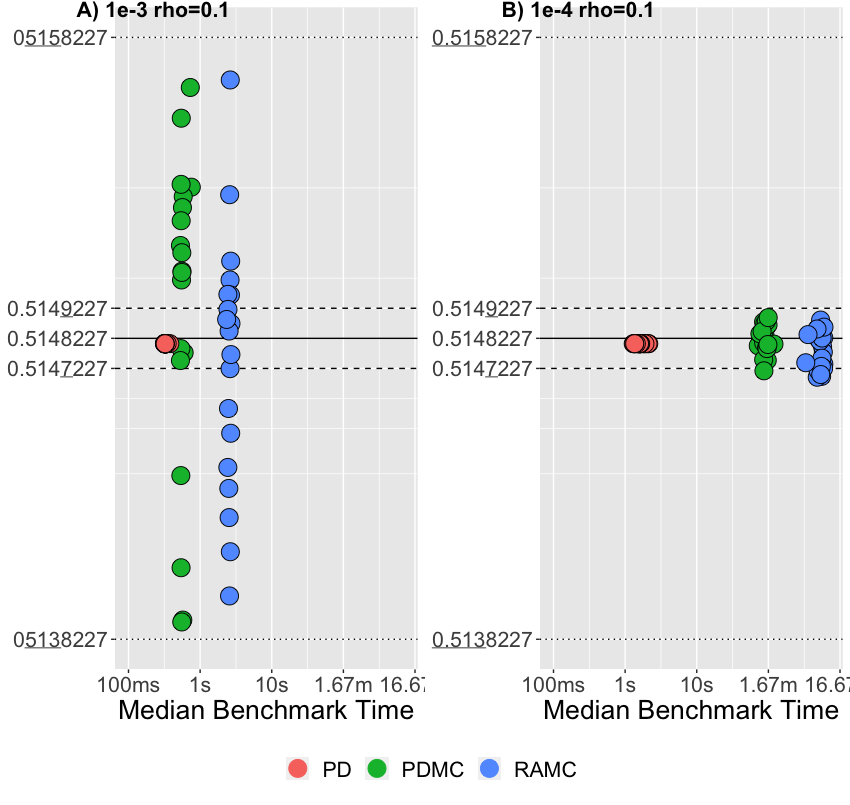
\includegraphics[scale=0.250]{supplemental_code/_04_precision_and_speed/d_004_alpha_1.70_Q_exch0.1_IL_same/Rplot_0.1.png}
  % 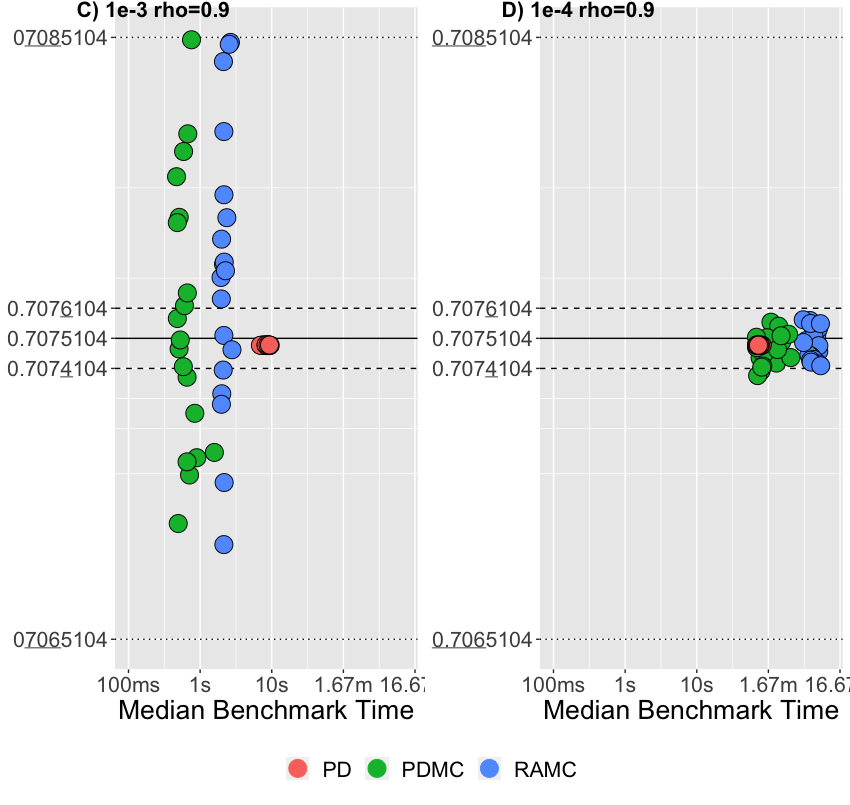
\includegraphics[scale=0.250]{supplemental_code/_04_precision_and_speed/d_004_alpha_1.70_Q_exch0.9_IL_same/Rplot_0.9.png}
%  \includegraphics[scale=0.25]{supplemental_code/_04_precision_and_speed/screen_shot_both.png}
  \includegraphics[height=3in, width=5.5in]{screen_shot_both.png}
  \caption{Speed and accuracy of distribution calculations.  Consider
    a multivariate subgaussian stable distribution of $d=4$,
    $\alpha=1.7$, with limits of integration being (-2,2) for each
    dimension.  In panels A) and B) we have an exchangeable shape
    matrix with $\rho=0.1$, and specified precision of 1e-3 and 1e-4
    for \code{pmvss} (PD), respectively.  Analogously, panels
    C) and D) display results for an exchangeable shape matrix with
    $\rho=0.9$.  Concurrently in each panel, are the results for Robust
    Analysis' \code{pmvstable.MC} (RAMC) and \code{pmvss\_mc}
    (PDMC) with enough simulated variates to produce a 95\ CI width
    that matches the precision. Each point is an independent call and
    the calculated distribution is on the Y-axis vs the median
    benchmark time on the X-axis. There are 20 calls per
    function per scenario. The dotted line is the 1e-3 boundary of the
    gold standard and the dashed line is the 1e-4 boundary. }
  \label{fig:speedacc1}
\end{figure}



\section{Bonus:  faster distribution calculations via a modified
  \code{QRSVN} algorithm}



\subsection{Insight: multivariate student's t
  distributions are a product distribution \label{sect:A:invgamma}}

The derivation of the univariate student's t distribution is commonly motivated
with a ratio of two quantities each involving random variables: a
standard normal $Z$ in the numerator and a $V \sim \chi^2(\nu)$ in the
denominator:
$$ T_\nu = \frac{Z}{\sqrt{V/\nu}} = Z\sqrt{ \frac{\nu}{V}} \,,$$
but what often is left out of the instruction is that
$A_\nu = \frac{\nu}{V} \sim IG\left( \frac{\nu}{2},
  \frac{\nu}{2}\right)$ has an inverse-gamma distribution, where
$X \sim IG\left(r, s \right)$ with rate $r$, shape $s$, and density
$f(x; r, s) = \frac{r^s}{\Gamma(s)}x^{(-s-1)} e^{-r/x}$.  This implies
we equivalently have a product distribution of the type
$T_\nu = A^{1/2}_\nu Z$.  This notion holds for the multivariate case
as well, where for $G \sim MVN( 0, Q)$ as before and $A_\nu$ is an
inverse-gamma with $r=s=\nu/2$
%% $$ A \sim IG\left( \frac{\nu}{2}, \frac{\nu}{2}\right)$$ 
then $H_\nu=A_\nu^{1/2} G$ is a $d$-dimensional student's t
distribution with $\nu$ degrees of freedom and covariance matrix $Q$.
This corresponds to Example 16 in in \citet{hamdan2000characterizing},
and is equivalent to the `chi-normal' ($\chi$-$\Phi$) formulation in
\citet{genz2002comparison} (earning the namesake `$\chi$` due to the
fact that $V \sim \chi^2(\nu) \implies \sqrt{V} \sim \chi(\nu)$).  For
$d \ge 4$, the QRSVN algorithm (\url{https://www.math.wsu.edu/faculty/genz/software/fort77/mvtdstpack.f)} is used in \code{mvtnorm::pmvt}.  The
reordering and rotational methodology that makes \code{pmvtnorm::pmvt}
so fast is independent of the part that generates $\sqrt{1/A_v}$
random variates. This means that if one replaced $\sqrt{1/A_v}$ with
$\sqrt{1/A}$ variates, \code{mvtnorm::pmvt} would produce \emph{not}
multivariate student's t distributions but \strong{multivariate
  subgaussian stable distributions}.  We implement a modified QRSVN
algorithm for multivariate subgaussian stable distributions in a
separate package, \CRANpkg{mvgb} in honor of Genz and Bretz.


\subsection{Implementation of \code{mvgb::pmvss} \label{sect:imp2}}



Generating random variates of $A$ requires two independent uniform
random variates, and only one of which is Quasi-Random in our
implementation.  Regardless, this modified QRSVN approach enables the
potential advantage of the rotation of the distribution and the
reordering of integration limits.
% If interested, consult the
% supplementary materials to learn more on how this modification was
% made.
The takeaway is, that for similar precision,
\code{mvgb::pmvss} may be much faster than \code{mvpd::pmvss}, such as
10 seconds vs 500 seconds for 4 digits of precision in the following
example:


\begin{example}
  R> set.seed(321)
  R> library(mvgb)
  R> tictoc::tic() 
  ## probability calculated by mvgb takes about 10 seconds
  R> gb_4digits <-
  +   mvgb::pmvss(lower = rep(-2,5),
  +               upper = rep( 2,5),
  +               alpha = fitmv$mult_alpha,
  +               Q = fitmv$mult_Q_posdef,
  +               delta = fitmv$univ_deltas,
  +               abseps = 1e-4,
  +               maxpts = 25000*350)
  R> tictoc::toc()
  9.508 sec elapsed
  > gb_4digits
  [1] 0.6768
  ## now calculate same probability with similar precision
  ## in mvpd
  R> tictoc::tic()
  ## probability calculated by mvpd takes about 10 MINUTES
  R> pd_4digits <-
  +   mvpd::pmvss(lower = rep(-2,5),
  +               upper = rep( 2,5),
  +               alpha = fitmv$mult_alpha,
  +               Q = fitmv$mult_Q_posdef,
  +               delta = fitmv$univ_deltas,
  +               abseps.pmvnorm = 1e-6,
  +               maxpts.pmvnorm = 25000*1000,
  +               abs.tol.si = 1e-4)
  R> tictoc::toc()
  518.84 sec elapsed
  R> pd_4digits[1]
  [1] 0.6768
\end{example}

Although currently on CRAN, we include \code{mvgb::pmvss} here as a
proof-of-concept and as an area of future work.  More research is
needed into its computational features and accuracy, and this is
encouraged by promising preliminary results.  Additionally, more
research may be warranted for other R package methodologies that use a
multivariate Gaussian, Cauchy, or Holtsmark distribution to generalize
to a multivariate subgaussian stable distribution (a helpful reviewer
suggested generalizing the multivariate distributions as used in
\CRANpkg{fHMM} \citep{oelschlager2021detecting} and generalizing the
normally mixed probit model in \CRANpkg{RprobitB}).  For more about
elliptically contoured multivariate distributions in general, consult
\cite{fang1990statistical, fang2018symmetric}.


\section*{Acknowledgements}
%Blinded.
This work utilized the computational resources of the NIH HPC Biowulf
cluster (http://hpc.nih.gov).  We thank Robust Analysis for providing
their \pkg{stable} \code{R} package via a software grant. 





%\section{Another section}
%
%There will likely be several sections, perhaps including code snippets, such as:
%
%\begin{example}
%  x <- 1:10
%  result <- myFunction(x)
%\end{example}
%
%\section{Summary}
%
%This file is only a basic article template. For full details of \emph{The R Journal} style and information on how to prepare your article for submission, see the \href{https://journal.r-project.org/share/author-guide.pdf}{Instructions for Authors}.

\bibliography{swihart-nolan.bib}

\address{Bruce J. Swihart\\
  National Institutes of Health \\
  National Institute of Allergy and Infectious Diseases\\
  5601 Fishers Lane Baltimore MD, 20852\\
  United States of America\\
  (ORCiD 0000-0002-4216-9942)\\
  \email{bruce.swihart@nih.gov}}

\address{John P. Nolan\\
  American University\\
  Department of Math \& Statistics \\
  4400 Mass. Ave, Washington DC 20016 \\
  United States of America\\
  (ORCiD 0000-0002-9669-382X)\\
  \email{jpnolan@american.edu}}
